\cleardoublepage
\chapter{Preliminaries}

\todo{

ACID vs CAP. What's consistency? What's isolation? What is a consistency guarantee?

Causal consistency. Vector clocks? Happens-before relationship

What's a transaction. Follow \textsection 3 in GMU paper

Explain the different levels of consistency (at least mention RC and SER, so we can talk about them during the evaluation) with the framework presented in Andrea/Alexey's CONCUR'15 paper (A Framework for Transactional Consistency Models with Atomic Visibility), using anomalies and abstract executions.

Re: rationale. The reason for our prefix is so that we could build static analysis on top. (see the `Robustness against...' paper for this.)
}

We begin with an introduction to the notation and basic concepts used throughout this thesis. We also review several \emph{strong} and \emph{weak} consistency models, based on the anomalies that are observable in each model. Finally, we discuss several protocols implementing some of these models, representing the previous work against which we compare our approach.

\section{Notation}

In this section, we define the elements we use throughout this chapter, such as transactions, histories, and relations. We follow the models used by Ardekani~\citep{ardekani_thesis}, Adya~\citep{adya_thesis} and Bernstein et al.~\citep{bernstein_concurrency}.

\subsection{Objects and Transactions}

We consider a database storing \textbf{\em objects} $\Obj = \{x, y, \ldots\}$, which we assume to be integer-valued. Clients interact with the database via \textbf{\em transactions} $\Trans = \{\tx_i \mid i \in \mathbb{N}\}$, with $i$ being the \emph{transaction identifier} of $\tx$. A transaction is a totally ordered sequence of read or write operations, followed by a \emph{terminating} operation: either commit or abort. This order follows the order in which the client invoked such operations. Given an object $x$ and a transaction $\tx_i$, we call $x_i$ to the \textbf{\em version} $i$ of $x$ written by $\tx_i$. We denote by $w_i(x_i)$ when a transaction $\tx_i$ writes a version $i$ of $x$, and $r_i(x_i)$ when $\tx_i$ reads a version $i$ of $x$. Finally, we denote by $c_i$ when $\tx_i$ commits, and $a_i$ when it aborts. We assume an initial transaction $\tx_0$ writes the initial versions of every object in the database. Without loss of generality, we also assume that no transaction performs \emph{blind updates}, that is, for every write operation $w_i(x_i)$ performed by $\tx_i$, there's always a preceding read operation $r_i(x_i)$. We say that a transaction is \textbf{\em read-only} if its set of operations does not include writes, and \textbf{\em update} otherwise.

\subsection{Histories}

We call a \textbf{\em history} $h$ to the finite set of all transactions with disjoint identifiers issued against a database. We denote the set of all possible histories by $\Hist$. For some history $h$, $\hb_h$ denotes a \textbf{\em happens-before} strict partial order over $h$, such that for any two transactions $\tx_i$ and $\tx_j$, if $w_i(x_i)$ and $r_j(x_i)$, $\tx_i \hb_h \tx_j$ (that is, $\tx_j$ reads the version $i$ of $x$ written by $\tx_i$). Intuitively $\tx_i \hb_h \tx_j$ means that $\tx_j$ is aware of the updates performed by $\tx_i$, and thus the outcome of the operations in $\tx_j$ may depend on the effects of $\tx_i$. In this case, we say that $\tx_i$ is a \textbf{\em causal dependency} of $\tx_j$. We can represent the history and the relations between operations and transactions as a graph, following Bernstein et al~\citep{bernstein_concurrency}.

\begin{figure}[h]
  \centering
  \vspace{-0.4cm}
  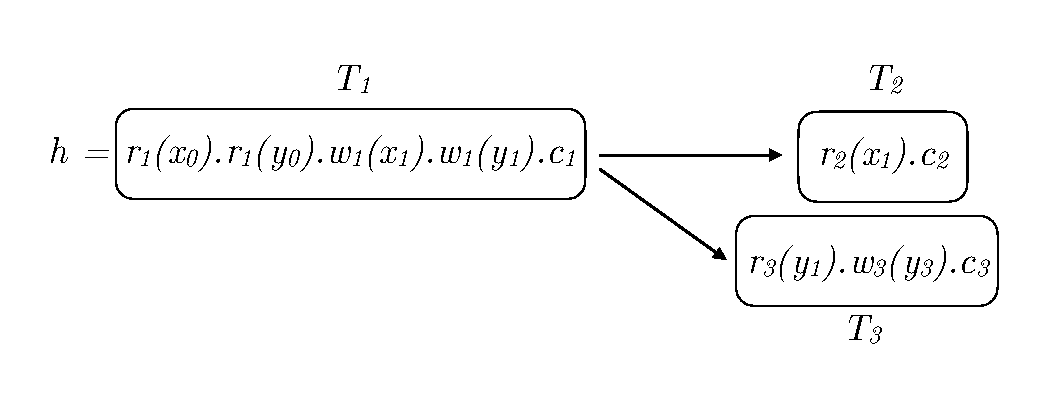
\includegraphics[width=0.7\textwidth]{figures/history.pdf}
  \vspace{-1cm}
  \caption{Example of history represented as a graph. Arrows represent the causal dependencies between operations. Adapted from \em{Ardekani et al.~\citep{ardekani-nsmi}}}
  \label{fig:history}
\end{figure}

Figure~\ref{fig:history} above shows an example, with $\tx_1 \hb_h \tx_3$ and $\tx_1 \hb_h \tx_2$. We say that two transactions $\tx_i$ and $\tx_j$ are \textbf{\em concurrent} in $h$ (denoted by $\tx_i \parallel \tx_j$) if neither $\tx_i \hb_h \tx_j$ nor $\tx_j \hb_h \tx_j$. In the figure above, $\tx_2$ and $\tx_3$ are concurrent.

\section{Consistency Models}

In this section, we define what a consistency model is, along with several related concepts. We distinguish between \emph{strong} and \emph{weak} models, and give definitions for both classes. We give an overview of several models, and compare them in terms of their undesirable effects.

We define a consistency model as a set of histories $\Cons$, such that $\Cons \subseteq \Hist$. Intuitively, a consistency model \emph{constrains} the set of possible histories by specifying how operations interleave in any given history. We say that a given history $h$ \emph{satisfies} a consistency model $\Cons$ if $h \in \Cons$, and that $h$ \emph{violates} $\Cons$.

In the context of databases, the definition of a consistency model maps to the concept of an \emph{isolation level} (I in AC\underline{I}D), which specifies the degree to which concurrent transactions in a database are aware of each other~\citep{adya_thesis}. We will use the term consistency throughout this thesis, in accordance with Adya~\citep{adya_thesis}.

Traditionally, the different consistency models have been defined in terms of \emph{anomalies}~\citep{sql-critique}, that map to a set of undesirable histories that are observable by the system.

\begin{figure}[h]
\begin{center}
\begin{tabularx}{\linewidth}{ >{\centering}p{8cm} | *{5}{>{\centering}X}}
    & \multicolumn{5}{c}{Consistency Models} \tabularnewline \cline{2-6}
    \emph{Anomalies} & SER & SI & PSI & NMSI & RC \tabularnewline \hline
    Dirty Reads & x & x & x & x & x \tabularnewline
    Non-Repeatable Reads & x & x & x & x & \checkmark \tabularnewline
    Read Skew & x & x & x & x & \checkmark \tabularnewline
    \hline
    Dirty Write & x & x & x & x & x \tabularnewline
    Lost Updates & x & x & x & x & \checkmark \tabularnewline
    Write Skew & x & \checkmark & \checkmark & \checkmark & \checkmark \tabularnewline
    Long Fork & x & x & \checkmark & \checkmark & \checkmark \tabularnewline
    \hline
    Non-Monotonic Snapshot & x & x & \checkmark & \checkmark & \checkmark \tabularnewline
    Real-Time Violation & \checkmark & \checkmark & \checkmark & \checkmark & \checkmark \tabularnewline
\end{tabularx}
\end{center}
\caption{Anomaly Comparison of Consistency Models \emph{(x}:disallowed\emph{)}. Adapted from \em{Ardekani et al.~\citep{ardekani-nsmi}}}
\label{fig:Anomalies}
\end{figure}

\subsection{Serialisability}
\subsection{Snapshot Isolation}
\subsection{Parallel Snapshot Isolation}
\subsection{Non-Monotonic Snapshot Isolation}
\subsection{Read Committed}

\section{Catalog of Protocols}
\subsection{Walter}
\subsection{Jessy}
% \subsection{GMU} Tentative, since we don't talk about US in previous section
